% This textfile includes
% 3. Analysis procedures
%    ..
%    ..
%    ..
%    3.3 Event and Object selection
%    3.4 Data and MC comparison
%    3.5 Background estimation
%
\section{Pile-up reweighting}
At the typical luminosity provided by the LHC, it is common to reconstruct more than one vertex per event. The main event vertex is defined as the one with the highest sum of the $p_{T}^{2}$ of the associated tracks. The presence of additional interactions, known as pile-up (PU). 

The simulation generates the pile-up roughly to match the condiction in data, however there are still difference between the pile-up numbers in data and MC. It is neccesary to reweight pile-up distribtuions of MC samples to match the data more precisely. By applying a proper weight to each MC event according to the pile-up distribution from data, the MC samples can describe the data better. Fig.~\ref{fig:PUreweight} shows the number of vertices after pile-up reweighting in both two lepton channel.

\begin{figure}[hbtp]
  \centering
  \subfigure[Number of vertices in muon channel]{
    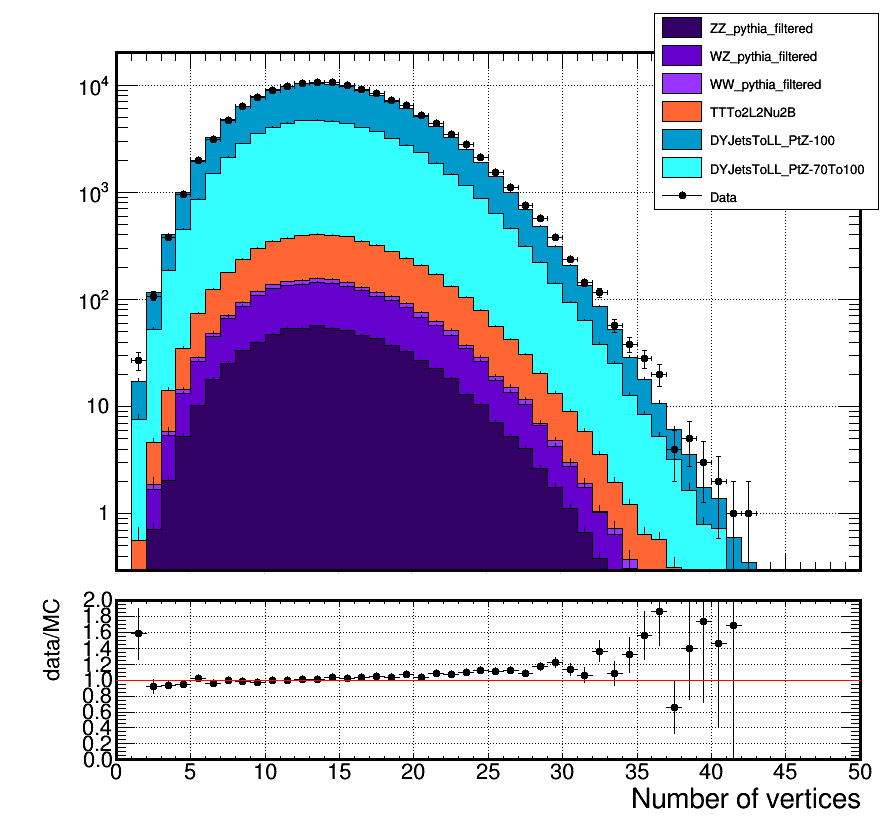
\includegraphics[scale=0.22]{figure/CH3/h_nVtx_Mu.png}}
  \hspace{0.5cm}
  \subfigure[Number of vertices in electron channel]{
    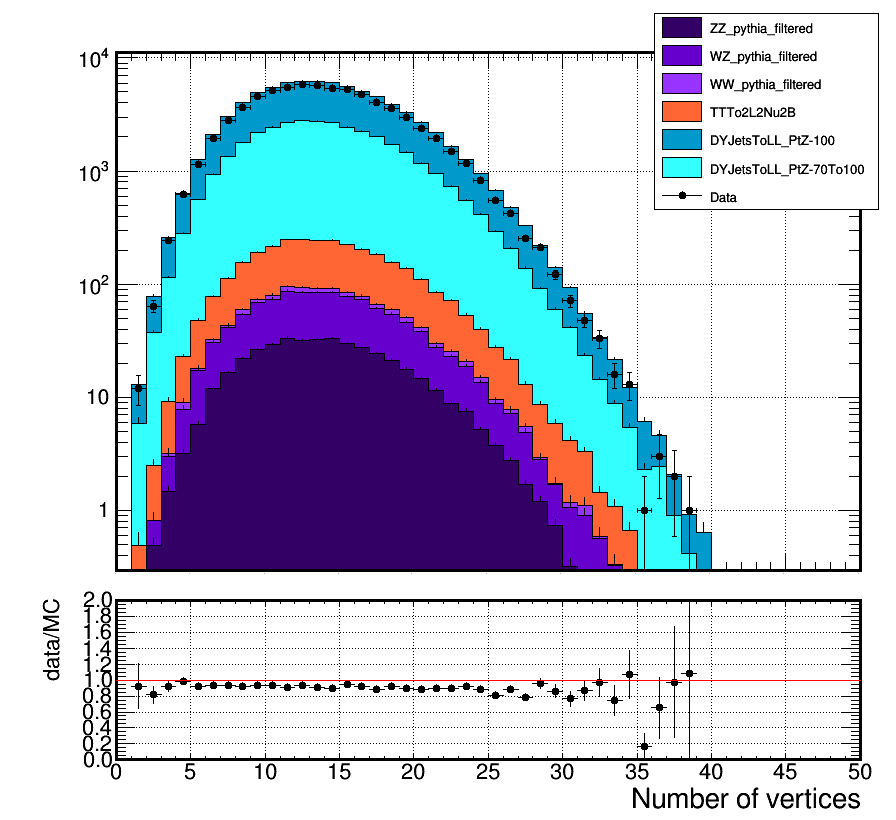
\includegraphics[scale=0.22]{figure/CH3/h_nVtx_El.png}}
  \caption{\label{fig:PUreweight}Number of vertices distributions after pile-up reweighting. Data are compared to the combination of all MC background samples. After reweighting, the distributions are almost identical to the data in both channels.}
\end{figure}



\newpage
\section{Event and Object selection}


\subsection{Lepton Requirements}

\subsection*{Muon Selection}

Besides the muon ID criteria disscussed in section 3.3.1 (table~\ref{tab:MuonIDtable}), we also require kinematic cuts on the muon candidates. We select the transverse momentum of the leading muon candidate must greater than 40 GeV, while the second leading muon transverse momentum threshold is 20 GeV. All muon candidates are must in the psuedo-rapidity $|\eta| < 2.4$ region.

\subsection*{Electron Selection}
Kinematic cuts on the electron candidates are also applied. Although the electron ID selection (table~\ref{tab:EleIDtable}) already required the pseudo-rapidity of electron supercluster, we cut on the $|\eta| < 2.5$ for electron candidates and all electrons must out of [1.4442,1.566] in the $\eta$ region to avoid the ECAL gap. The $p_{T}$ requirement is a bit different from the muon case. Since the HLT trigger already selects electron $p_{T}$ greater than 33 GeV, we require both leading and sub-leading electrons $p_{T}$ greater than 40 GeV in advance.

\subsection{Jet Requirement}
CA8jets in our signal process is originated from Higgs decay. If the $Z'$ mass is large enough, the Higgs will be boosted. Therefore we require higher kinematic thresholds to the CA8jets. In every event, there must find at least one CA8jet with $p_{T} > 80$ GeV, $|\eta| < 2.4$, passing loose jet ID and the pruned-jet mass must greater than 40 GeV to remove jets from backgrounds.

Futhermore, in order to veto leptons that are mis-identified as jets, leptons overlap with jets are removed by the $\Delta R$ cut, i.e. if there's a lepton passing all lepton selections and the spatial distance to a CA8jet smaller than 0.1 ($\Delta R_{jet,lepton} < 0.1$), then the jet will be removed.

\subsection{Z boson Requirement}
The Z boson candidate is reconstructed by adding four-momentum of the selected lepton pair. Since the Z boson mass is about 91 GeV, we require the reconstructed invariant mass of the Z boson in the mass region [70 GeV, 110 GeV] where is $\pm 20$ GeV to its theoretical mass.

For the CA8jet from Higgs, we require $p_{T}$ threshold as 80 GeV. The kinematics of reconstructed Z boson and Higgs should be symmetric, because they are both decayed from the heavy $Z'$, comparing their mass to $Z'$, the difference between 125 GeV and 91 GeV is negligible ($1\textup{ TeV} >> 125 \textup{ GeV} \sim 91 \textup{ GeV}$). Therefore we require the same $p_{T}$ theshold to the Z boson. Fig.~\ref{fig:genZHPt} shows the transverse momentum distributions from the signal samples.

\begin{figure}[hbtp]
  \centering
  \subfigure[generator level Higgs $p_{T}$ distribustion]{
    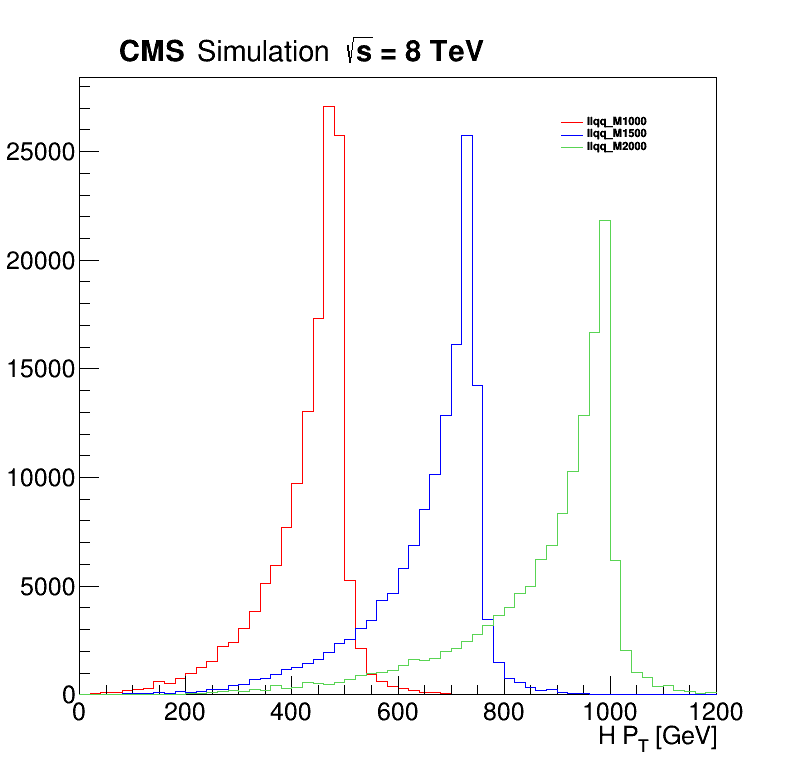
\includegraphics[scale=0.25]{figure/CH3/h_genHPt.png}}
  \hspace{0.5cm}
  \subfigure[generator level Z boson $p_{T}$ distribustion]{
    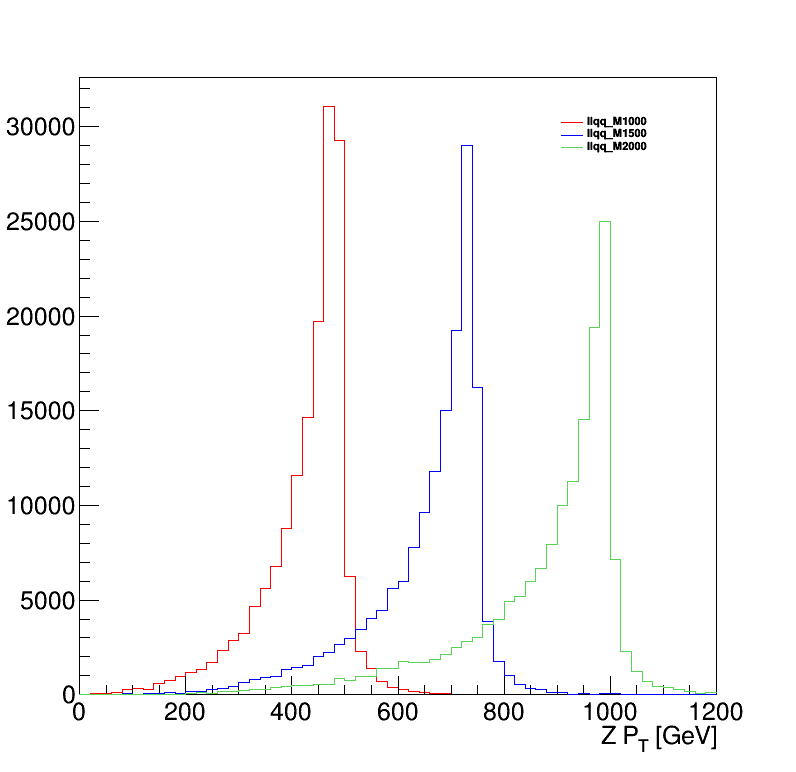
\includegraphics[scale=0.25]{figure/CH3/h_genZPt.png}}
  \caption{\label{fig:genZHPt}Z and Higgs $p_{T}$ distribution are almost identical. We pick three samples with different mass points of $Z'$, 1000 GeV (red), 1500 GeV (blue) and 2000 GeV (green). These plots are made from the generator level signal samples without any proper selections.}
\end{figure}

Finally, all selection requirements are summarized in table~\ref{tab:preselection}.
\newpage

\begin{center}
  \begin{table}[h]
    \begin{center}
      \begin{tabular}{|lcc|}
        \hline
        \textbf{Selection} & \textbf{Value} & \textbf{Comments} \\ \hline
        Trigger & HLT\_Mu22\_TkMu8 & DoubleMu dataset \\
        & HLT\_DoubleEle33 & DoublePhoton dataset \\ \hline
        Leading muon $p_{T}$ & $p_{T} > 40$ GeV &\\
        Sub-leading muon $p_{T}$ & $p_{T} > 20$ GeV &\\
        Muon $\eta$ & $|\eta| < 2.4$ &\\
        Muon ID & High $p_{T}$ tracker based &\\
        Muon isolation $I_{trk}^{mod}$ & $< 0.1$ &\\ \hline
        Leading electron $p_{T}$ & $p_{T} > 40$ GeV &\\
        Sub-leading electron $p_{T}$ & $p_{T} > 40$ GeV &\\
        Electron $\eta$ & $|\eta| < 2.5$ &\\
        & out of [1.4442,1.566] & To avoid ECAL gap. \\
        Electron ID & HEEP modified &\\
        Electron isolation  & &\\
        $I_{trk}^{mod}$ & $<$ 5 GeV &\\
        $I_{ECAL,HCAL}^{mod}$ & $<$ 2 GeV + 0.03$E_{T}$ & Barrel \\
        & $< 2.5$ GeV & for $E_{T} < 50$ GeV candidates in Endcap\\
        & $< 2.5$ GeV + 0.03$E_{T}$ & for $E_{T} > 50$ GeV candidates in Endcap\\ \hline
        Jet ID & Loose working point &\\
        Jet $p_{T}$ & $p_{T} > 80$ GeV &\\
        Jet $\eta$ & $|\eta| < 2.4$ &\\
        Prunedjet mass & $> 40$ GeV &\\
        Veto jet-lepton overlap & $\Delta R_{jet,lepton} < 0.1$ & Remove the jet satisfies this requirement.\\ \hline
        Z $p_{T}$ & $p_{T} > 80$ GeV &\\
        Z mass window cut & $70 \textup{ GeV} < M_{Z} < 110 \textup{ GeV}$ &\\
        \hline
      \end{tabular}
    \end{center}
    \caption{\label{tab:preselection}Event and object selection requirements used in the analysis.}
  \end{table}
\end{center}

\newpage
\section{Data-MC comparison}

In this section, a comparison between data and simulation is reported for various kinematic observables. It can be seen that the dominant background contribution comes from the Z+jets production, while sub-leading contributions are from $t\bar{t}$ and dibosons can be negligible.

On top of the selections described in previous section, additional regions are defined as following:

\begin{itemize}
\item \textbf{Signal region (SR)}: Represents the phase space where the signal is expected, defined by the prunedjet mass in $110 \textup{ GeV} < M_{prunedjet} < 140 \textup{ GeV}$ region. The range is chosen by $\pm$15 GeV to the mass of Higgs.
\item \textbf{Sidebands (SB)}: Defined by the interval between $70 \textup{ GeV} < M_{prunedjet} < 110 \textup{ GeV}$. This region is signal-depleted. In our case, we don't consider prunedjet mass higher than 140 GeV, because of the poor statistics and the excessive contribution of $t\bar{t}$ events.
\end{itemize}

In the following plots, the data-MC comparison is performed in SB region and all background samples are weighted to the same luminosity as data. Because the signal region in data is considered \textbf{blind} in this analysis stage, so they are not shown.

\begin{figure}[hbtp]
  \centering
  \subfigure[Muon energy fraction]{
    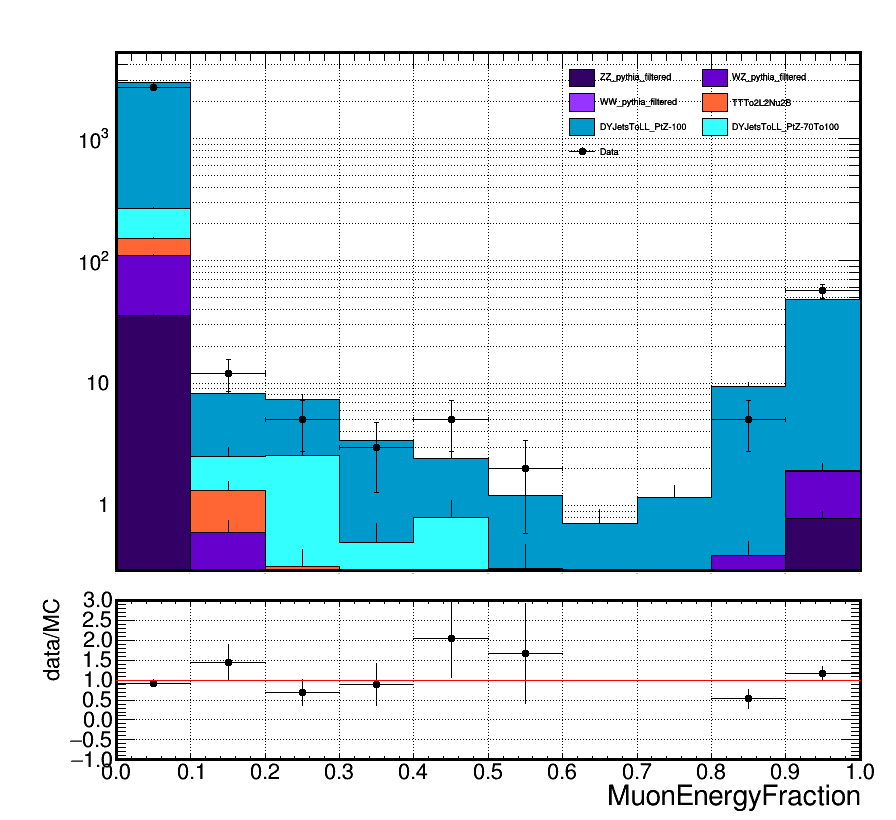
\includegraphics[scale=0.22]{figure/CH3/JetID/h_CA8jetMuEF.png}}
  \hspace{0.5cm}
  \subfigure[Photon energy fraction]{
    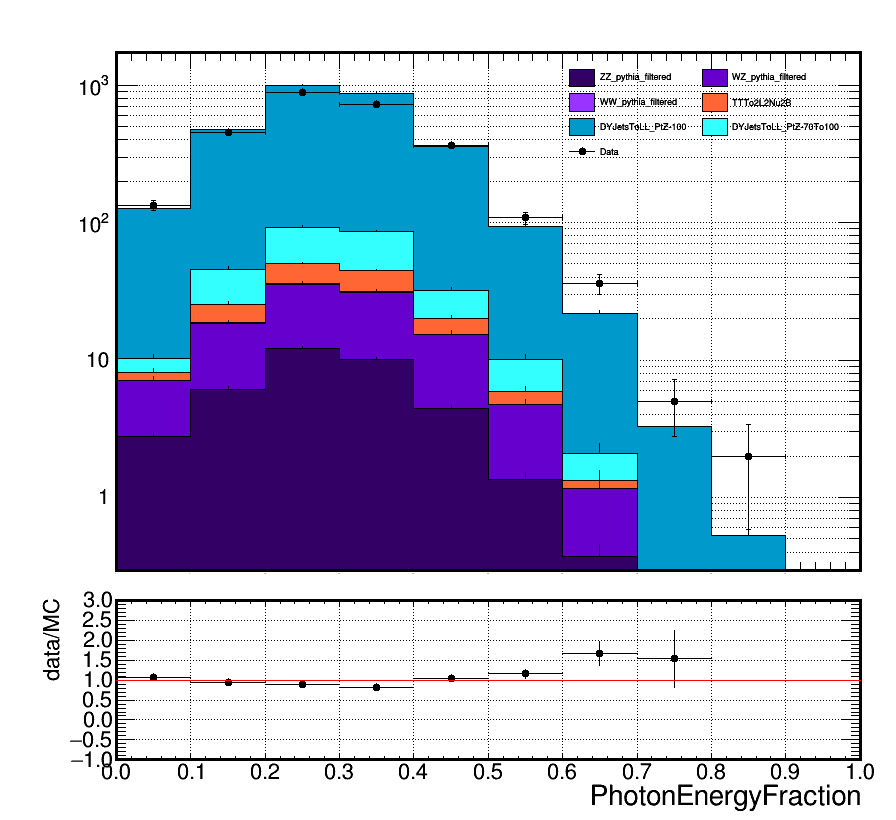
\includegraphics[scale=0.22]{figure/CH3/JetID/h_CA8jetPhoEF.png}}
  \caption{\label{fig:MuPhoEF}Comparison between data and all background samples for two jet variables. The definition of muon/photon  energy fraction is muon/photon energy divided by jet energy.}
\end{figure}

\begin{figure}[hbtp]
  \centering
  \subfigure[Charged electromagnetic energy fraction]{
    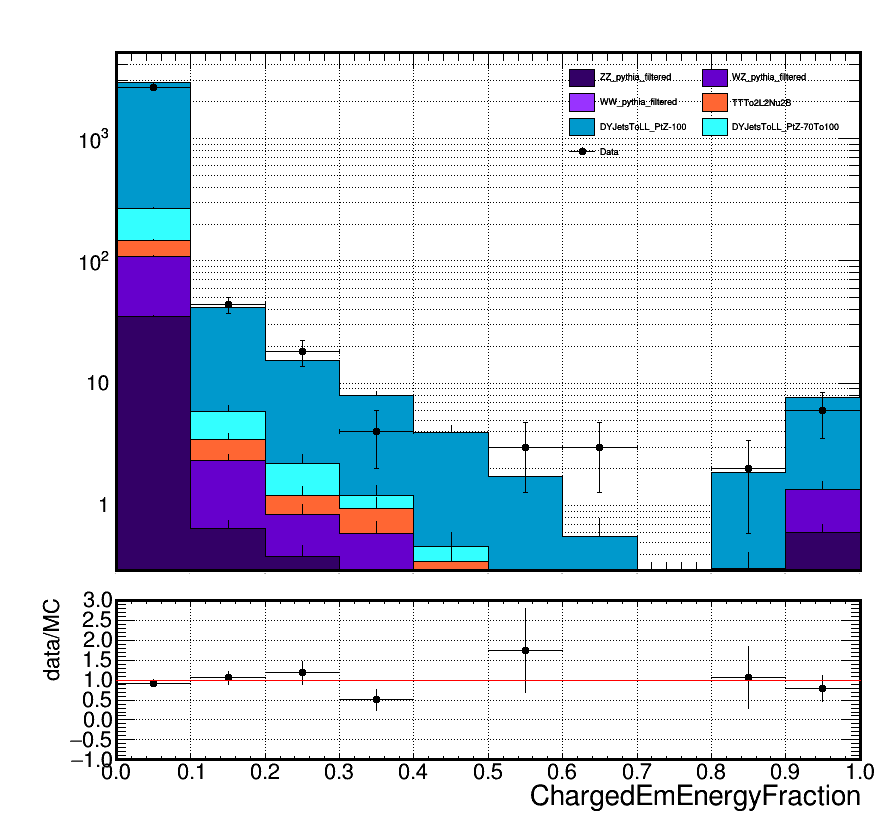
\includegraphics[scale=0.22]{figure/CH3/JetID/h_CA8jetCEmEF.png}}
  \hspace{0.5cm}
  \subfigure[Charged hadron energy fraction]{
    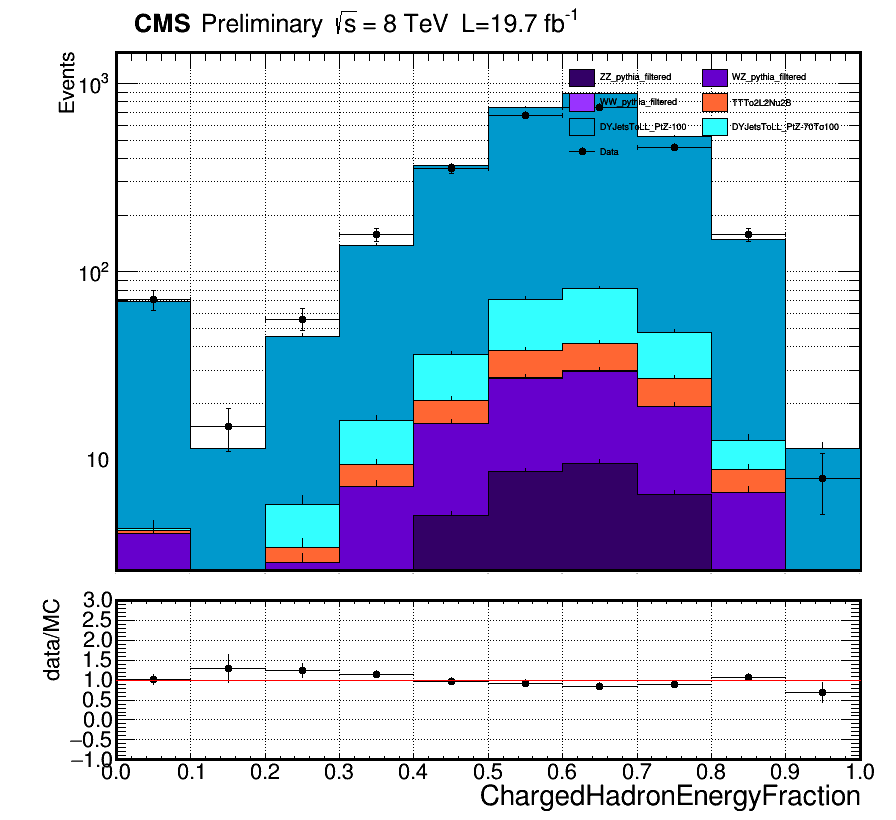
\includegraphics[scale=0.22]{figure/CH3/JetID/h_CA8jetCHadEF.png}}
  \caption{\label{fig:ChargedEF}Charged electromagnetic/hadron energy fraction is defined by the ratio of the energy of charged particles in ECAL/HCAL to the jet energy.}
\end{figure}

\begin{figure}[hbtp]
  \centering
  \subfigure[Neutral electromagnetic energy fraction]{
    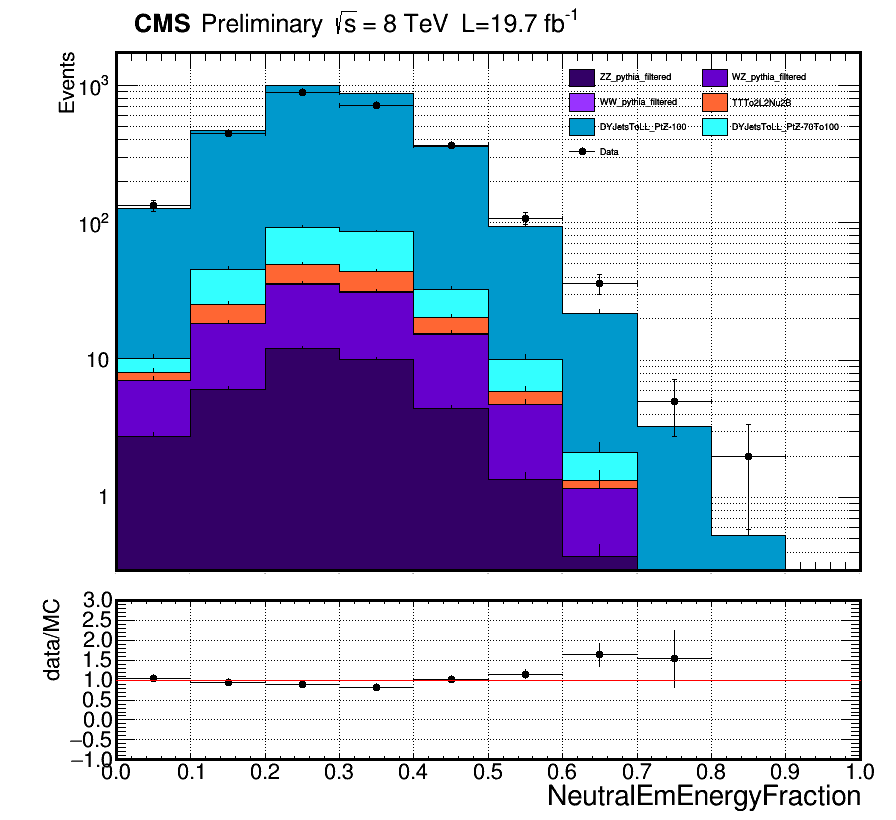
\includegraphics[scale=0.22]{figure/CH3/JetID/h_CA8jetNEmEF.png}}
  \hspace{0.5cm}
  \subfigure[Neutral hadron energy fraction]{
    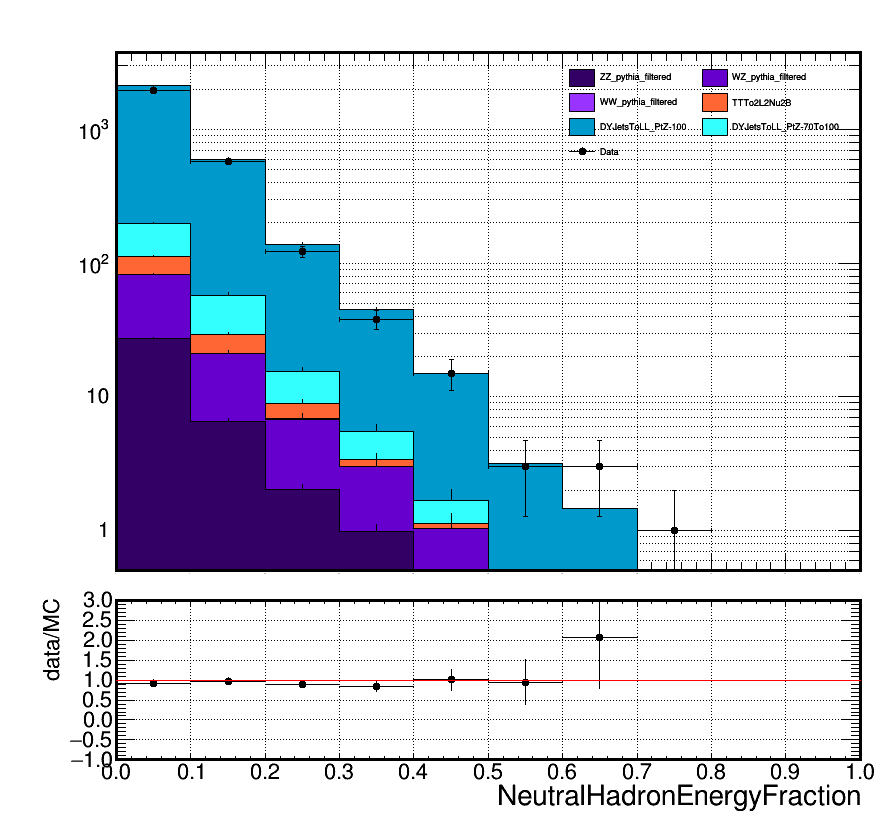
\includegraphics[scale=0.22]{figure/CH3/JetID/h_CA8jetNHadEF.png}}
  \caption{\label{fig:NeutralEF}Neutral electromagnetic/hadron energy fraction is defined by the ratio of the energy of neutral particles in ECAL/HCAL to the jet energy.}
\end{figure}

\begin{figure}[hbtp]
  \centering
  \subfigure[Jet multiplicity]{
    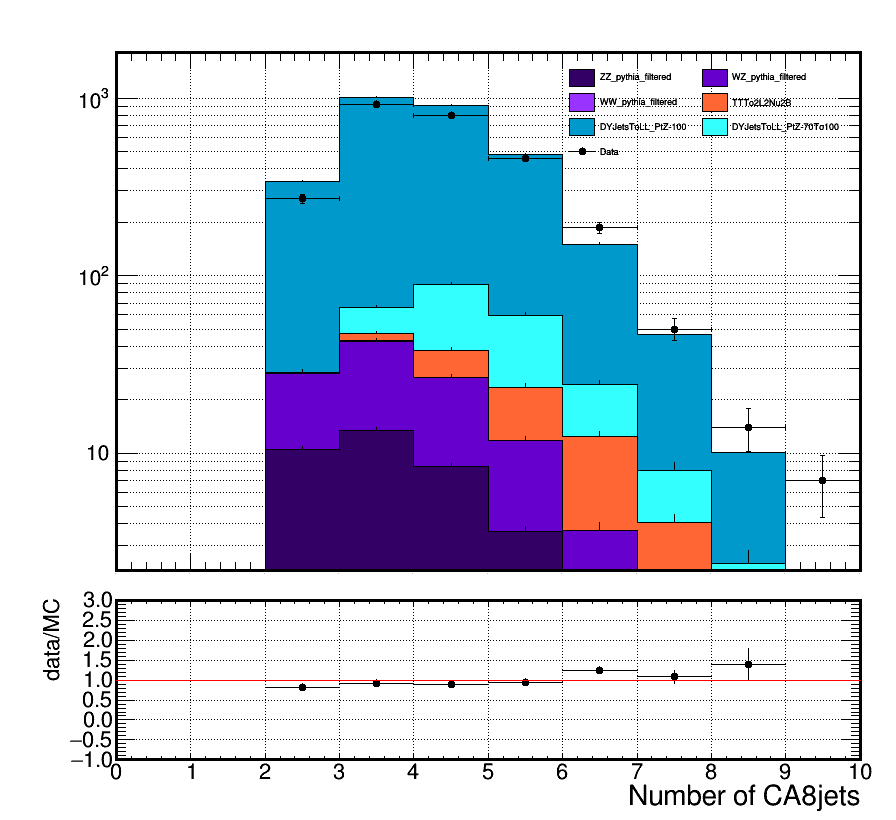
\includegraphics[scale=0.22]{figure/CH3/Jet_kinematics/h_nCA8jet.png}}
  \hspace{0.5cm}
  \subfigure[CA8jet $p_{T}$]{
    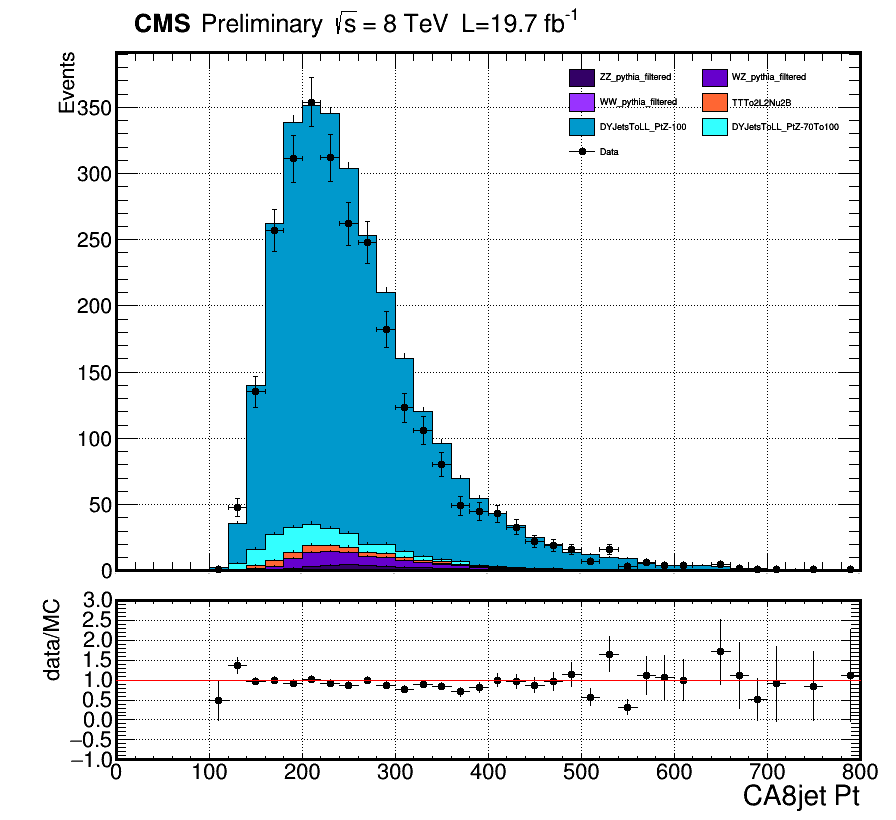
\includegraphics[scale=0.22]{figure/CH3/Jet_kinematics/h_CA8jetPt.png}}
  \caption{\label{fig:nCA8jetPt}Comparison between data and MC in SB region using jet multiplicity (number of jets) and CA8jet transverse momentum.}
\end{figure}

\begin{figure}[hbtp]
  \centering
  \subfigure[CA8jet $\eta$]{
    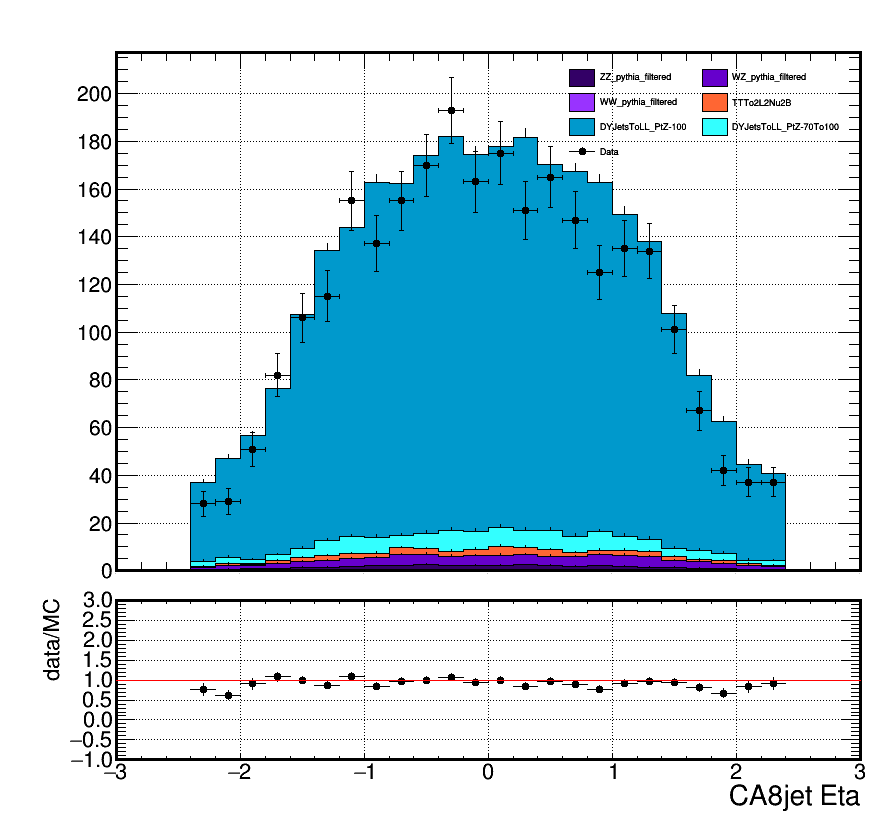
\includegraphics[scale=0.22]{figure/CH3/Jet_kinematics/h_CA8jetEta.png}}
  \hspace{0.5cm}
  \subfigure[CA8jet $\phi$]{
    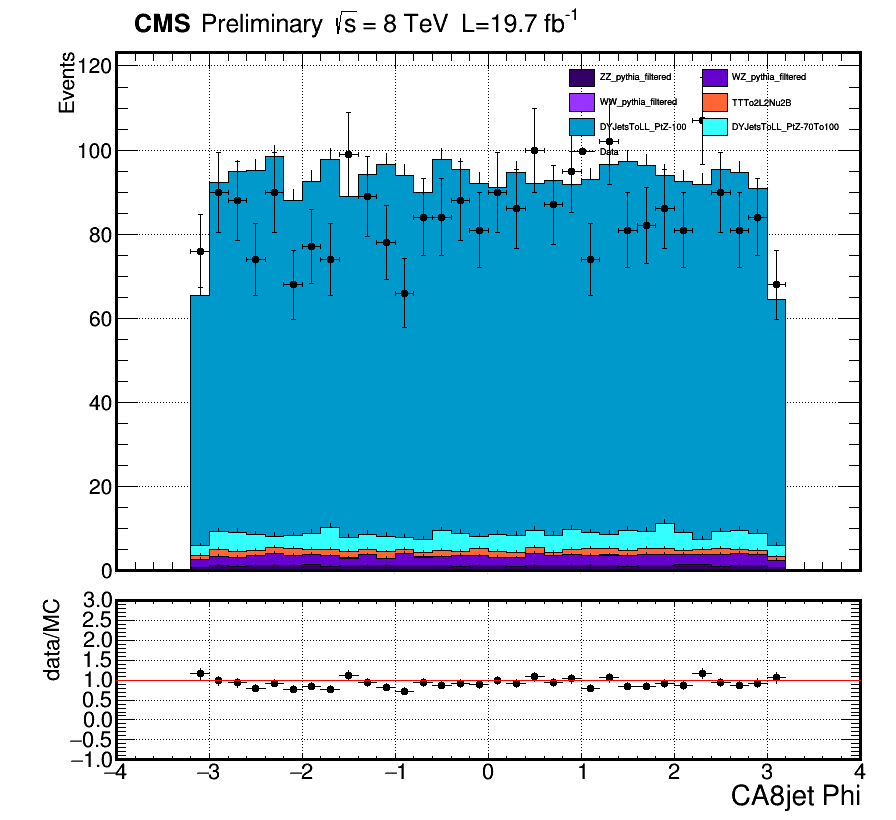
\includegraphics[scale=0.22]{figure/CH3/Jet_kinematics/h_CA8jetPhi.png}}
  \caption{\label{fig:CA8jetEtaPhi}Comparison between data and MC in SB region using CA8jet $\eta$ and $\phi$.}
\end{figure}

\begin{figure}[hbtp]
  \centering
  \subfigure[Prunedjet mass]{
    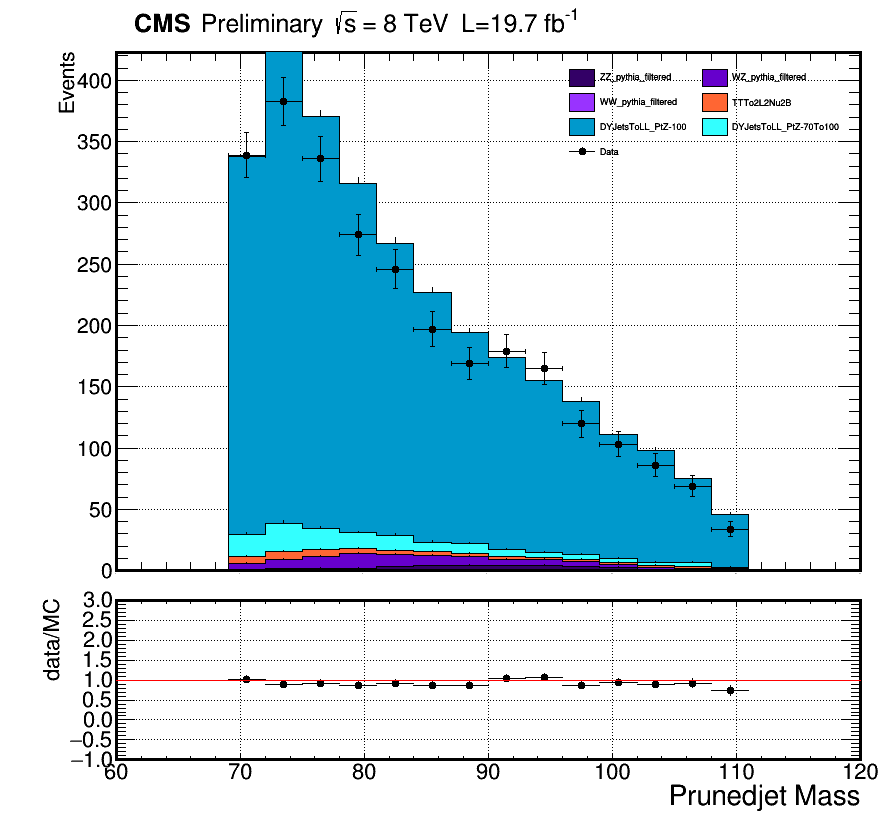
\includegraphics[scale=0.22]{figure/CH3/Jet_kinematics/h_PrunedjetM.png}}
  \hspace{0.5cm}
  \subfigure[$\Delta R$ between two subjets]{
    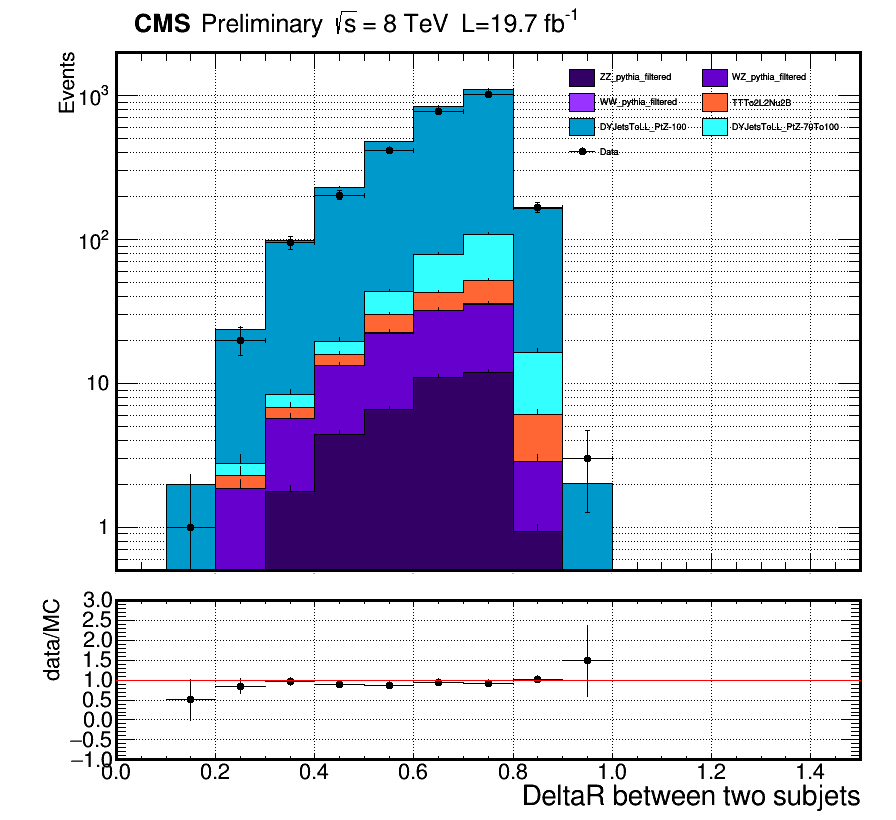
\includegraphics[scale=0.22]{figure/CH3/Jet_kinematics/h_DeltaRjj.png}}
  \caption{\label{fig:prunedmassDRjj}Left: the prunedjet mass in the SB region. Right: the spatial distance between two subjets within the CA8jet.}
\end{figure}

\begin{figure}[hbtp]
  \centering
  \subfigure[Z mass]{
    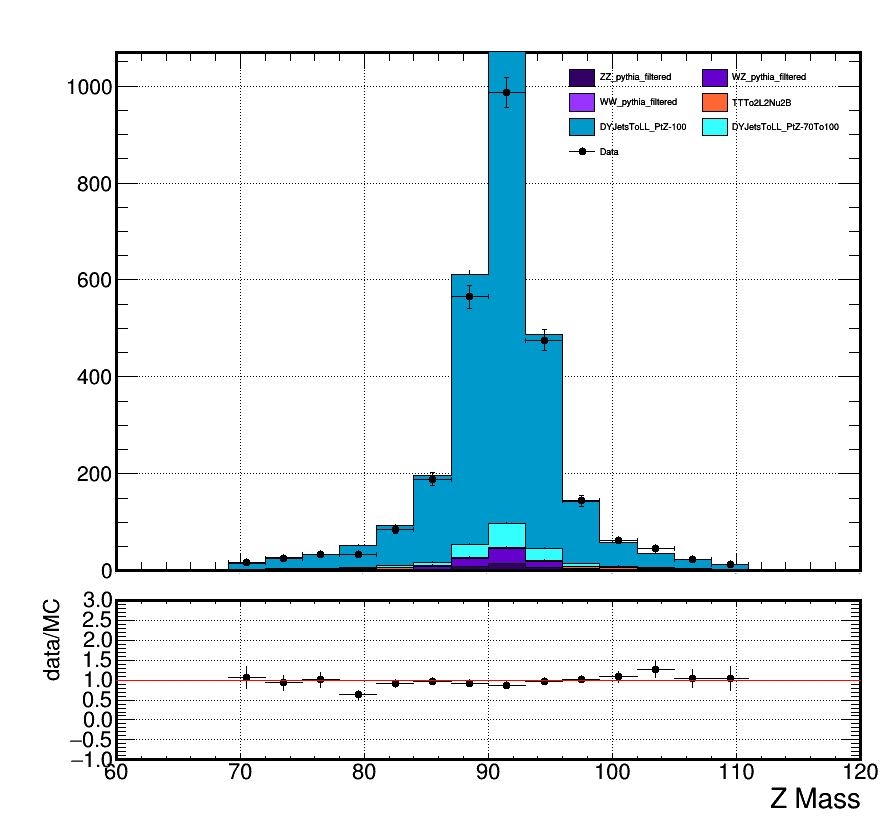
\includegraphics[scale=0.22]{figure/CH3/Z_kinematics/h_ZMass.png}}
  \hspace{0.5cm}
  \subfigure[Z $p_{T}$]{
    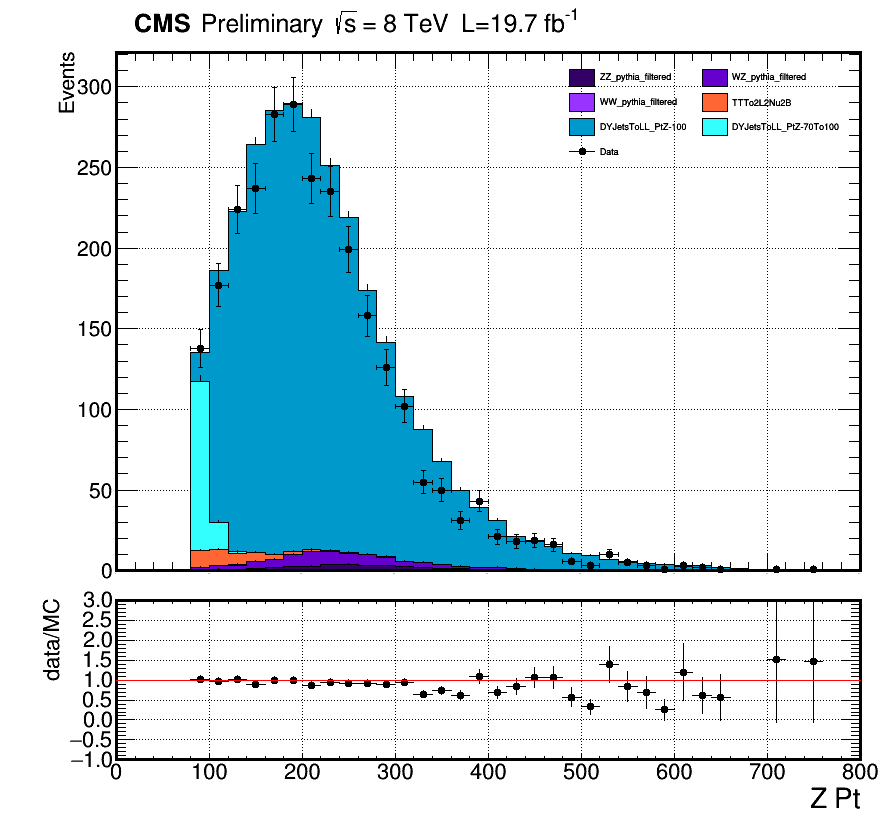
\includegraphics[scale=0.22]{figure/CH3/Z_kinematics/h_ZPt.png}}
  \caption{\label{fig:ZMassPt}Comparison between data and MC in SB region using mass and transverse momentum of reconstructed Z boson.}
\end{figure}

\begin{figure}[hbtp]
  \centering
  \subfigure[Z $\eta$]{
    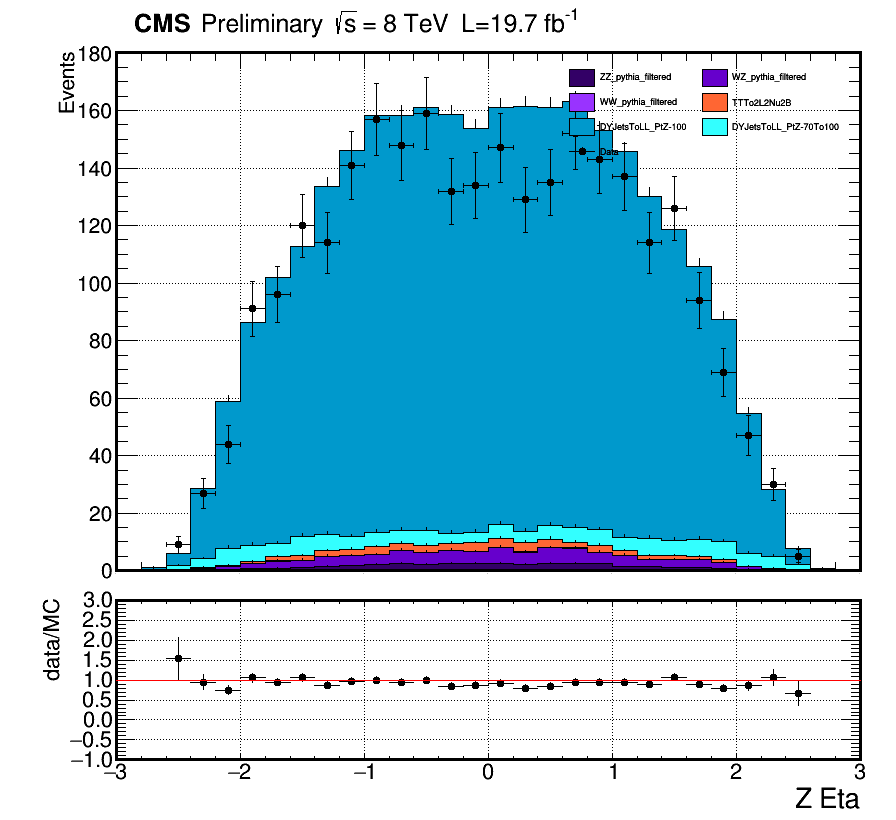
\includegraphics[scale=0.22]{figure/CH3/Z_kinematics/h_ZEta.png}}
  \hspace{0.5cm}
  \subfigure[Z $\phi$]{
    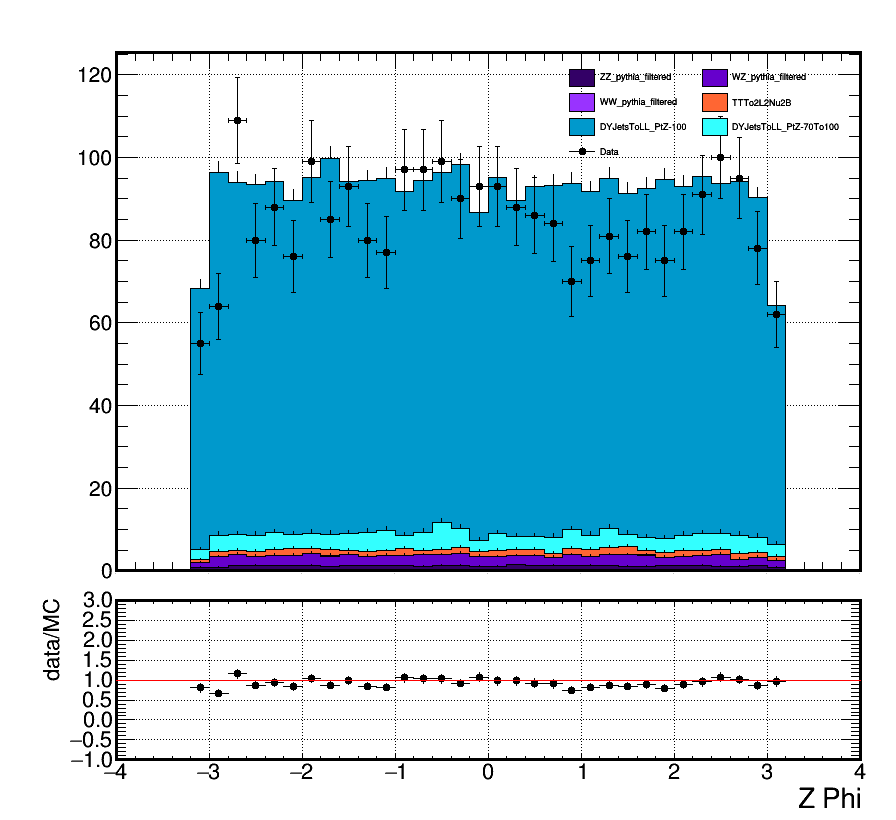
\includegraphics[scale=0.22]{figure/CH3/Z_kinematics/h_ZPhi.png}}
  \caption{\label{fig:ZEtaPhi}Comparison between data and MC in SB region using $\eta$ and $\phi$ of reconstructed Z boson.}
\end{figure}

\begin{figure}[hbtp]
  \begin{center}
    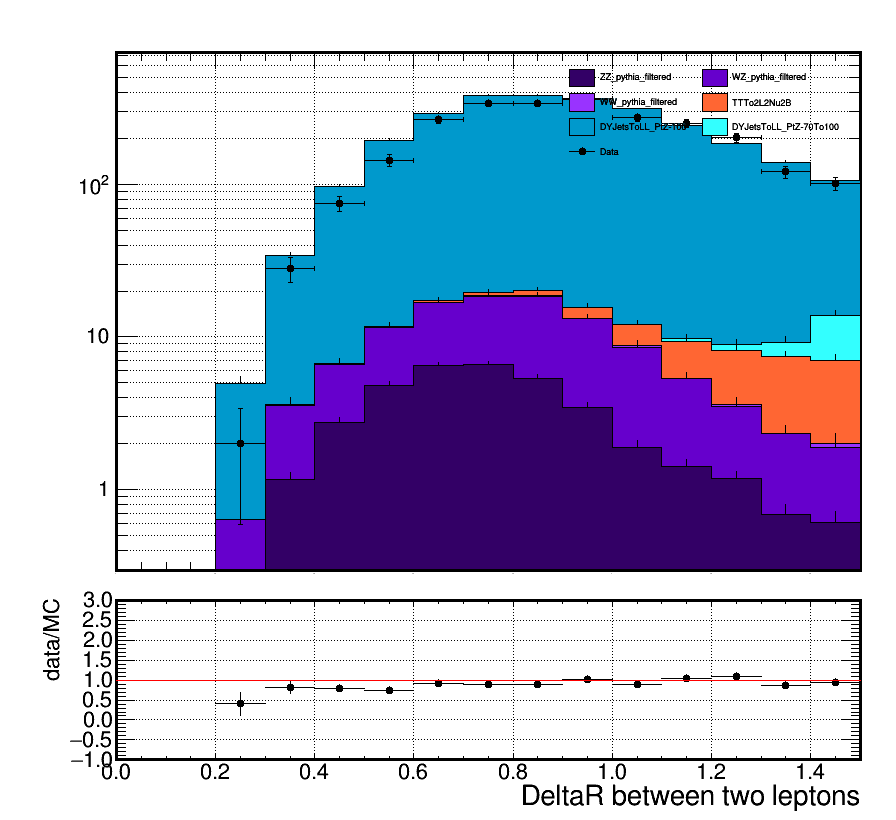
\includegraphics[width=0.5\textwidth]{figure/CH3/Z_kinematics/h_DeltaRll.png}
  \end{center}
  \caption{\label{fig:DeltaRll}$\Delta R$ between the two selected leptons.}
\end{figure}

\newpage
\section{Background Extrapolation}

The final aim of this analysis is to compare the predicted SM background with the observed data, it is important to elaborate a trustworthy strategy for the background estimation. Despite the good description of the event kinematics provided by the MC simulation, it is more advisable to minimize the dependence on the MC and develop a data driven strategy.


